\chapter{Methodology}
\label{Chapter3}

\section{Overall Framework}
The methodology enforces device-local authorization before execution and debug enablement.
The pipeline integrates (i) a custom ISA instruction (\texttt{kc}), (ii) protected key
storage in non-volatile memory, (iii) a constant-time comparator, (iv) a security FSM that
gates execution and debug access, and (v) toolchain support that emits the authorization
primitive in compiled binaries. The end-to-end workflow spans key binding on the host,
UART-based authorization sequencing, and on-device verification before privileged
capabilities are released. The overall flow is summarized in Fig.~\ref{fig:method-flow}.

\begin{figure}[H]
  \centering
  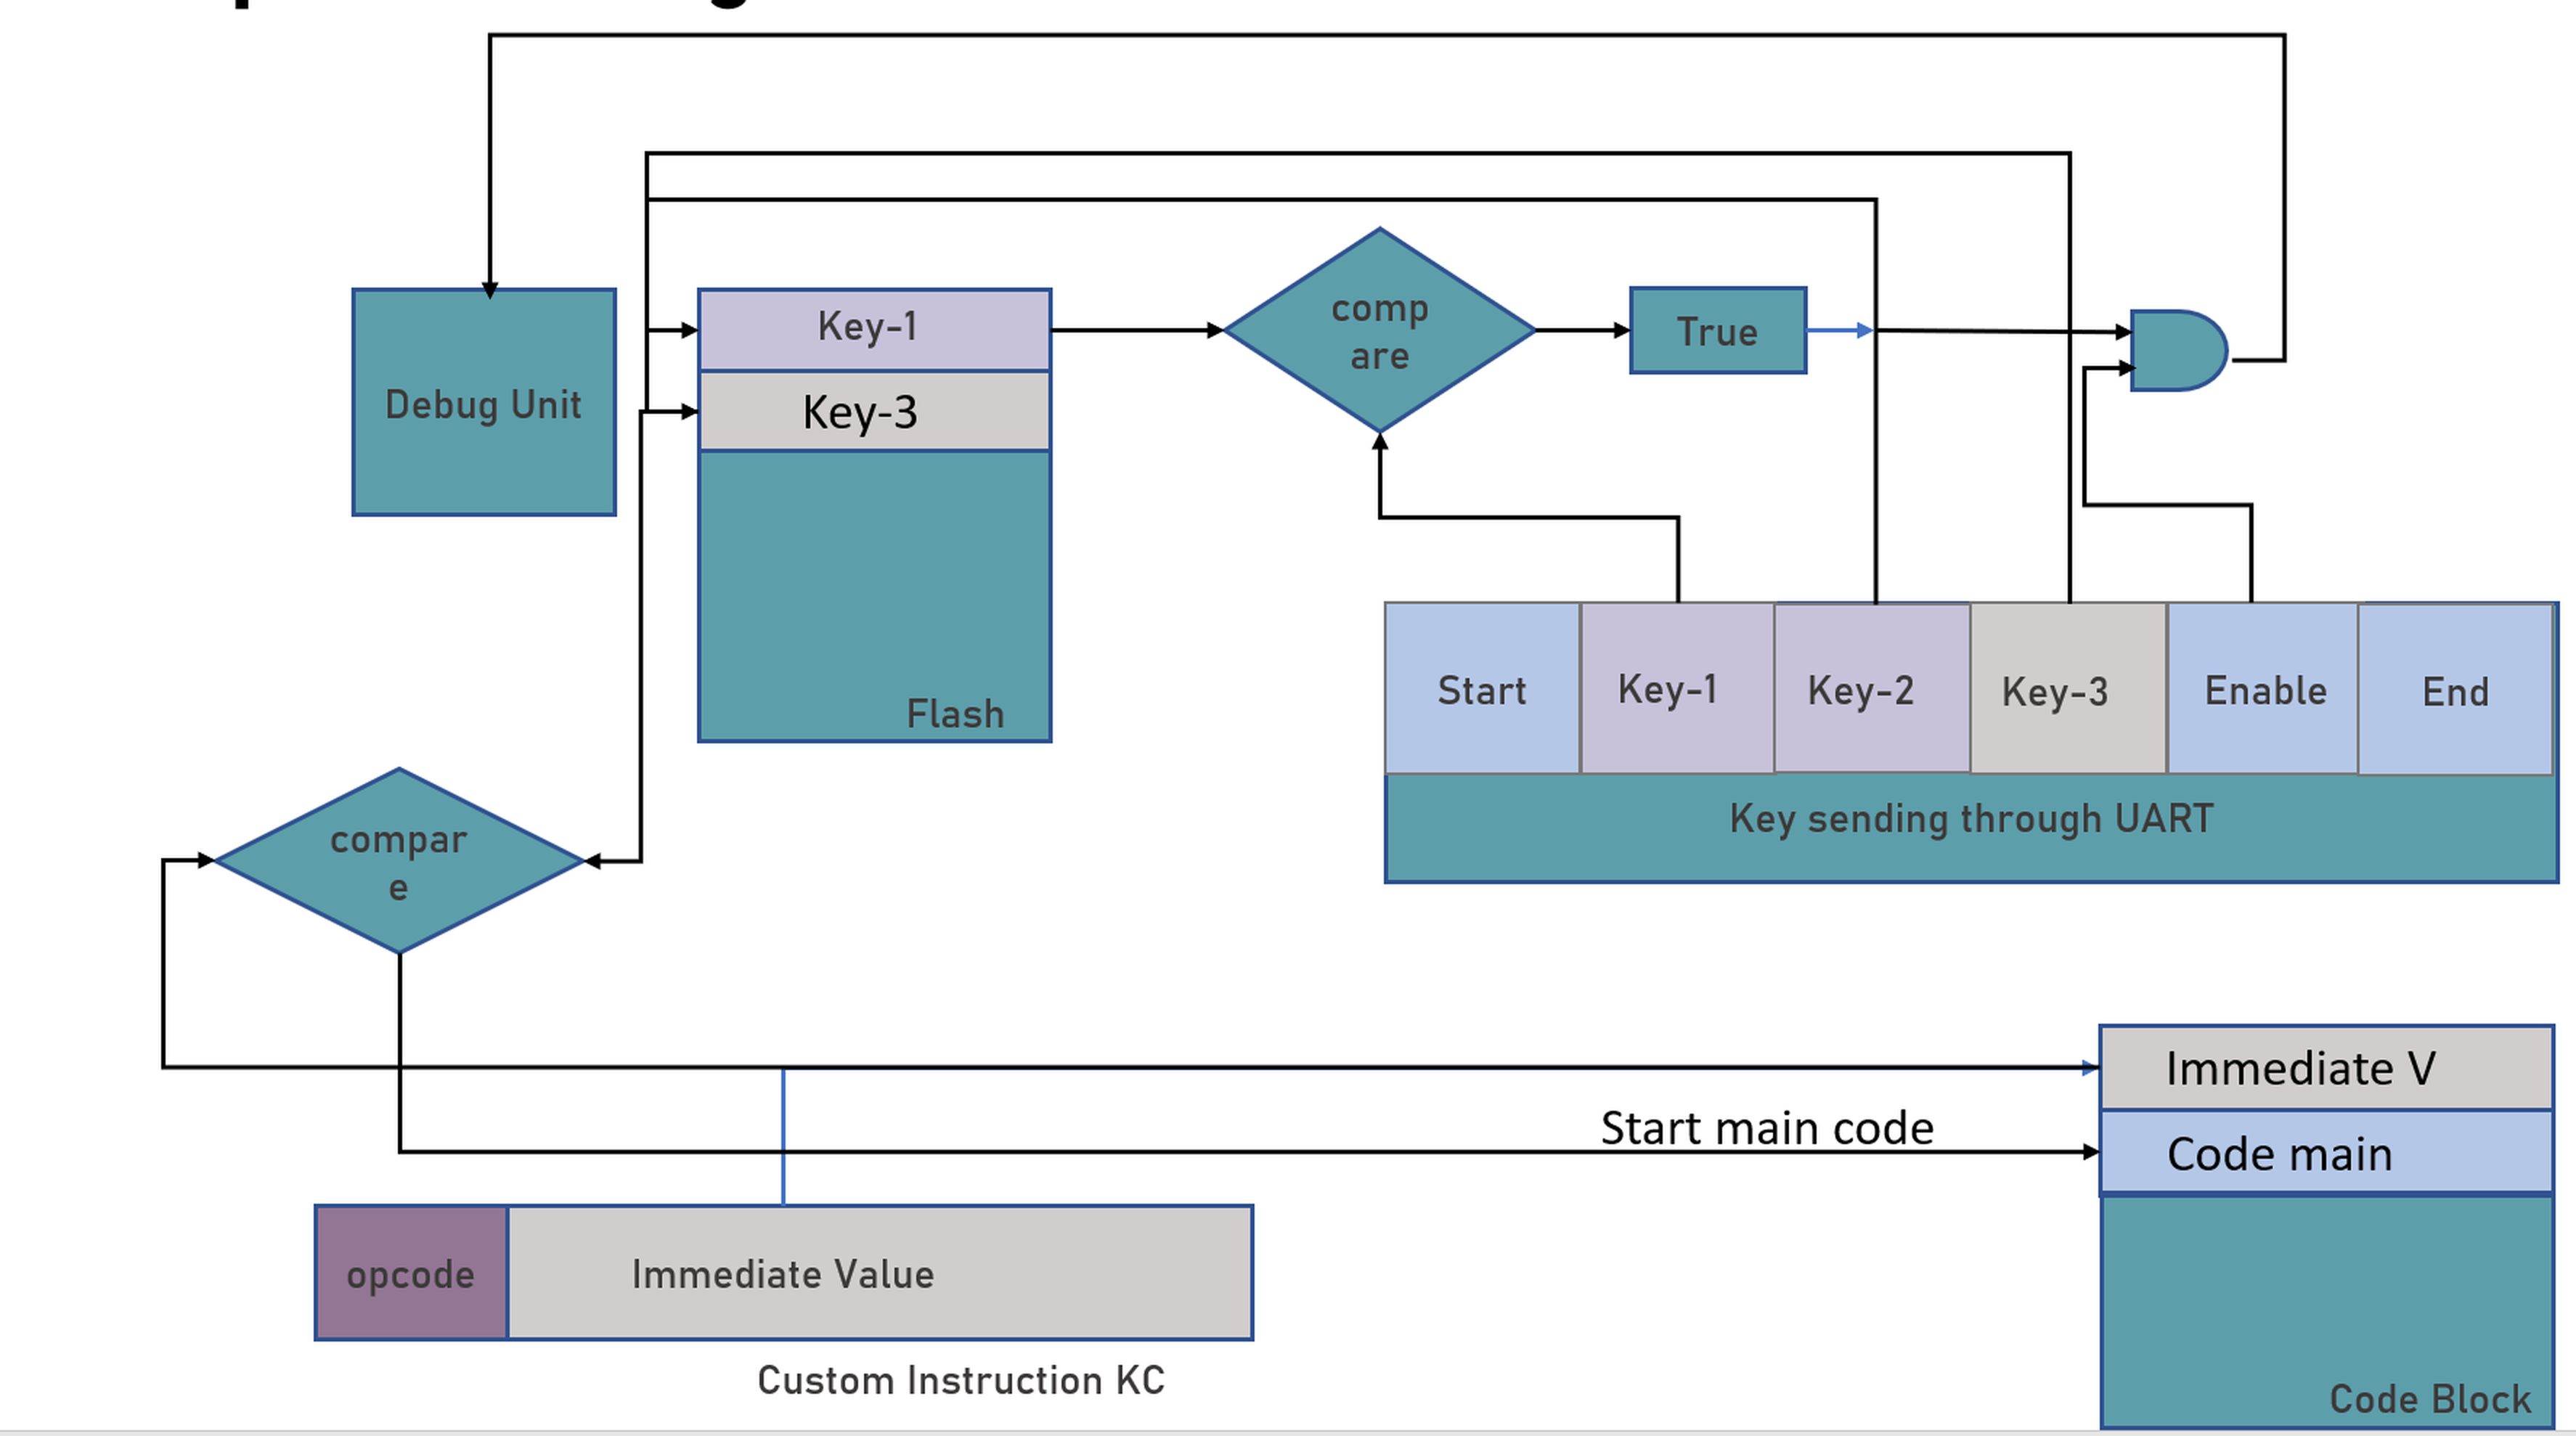
\includegraphics[width=0.95\linewidth]{figures/fig_arch_flow.png}
  \caption{Methodology flow: host workflow, UART authorization sequence, protected key
  storage, compare/verification, and ISA-level trigger via \texttt{kc}.}
  \label{fig:method-flow}
\end{figure}

\begin{table}[H]
  \centering
  \caption{Methodology pipeline summary}
  \label{tab:method-pipeline}
  \begin{tabular}{@{}p{3.2cm}p{4.6cm}p{4.6cm}@{}}
    \toprule
    \textbf{Stage} & \textbf{Input} & \textbf{Output} \\
    \midrule
    Key binding & Host/device identifiers, nonce & Device-bound key metadata \\
    Provisioning & Reference key in protected NVM & Non-mapped key storage \\
    Authorization sequence & Start, Key-1..Key-3, Enable & UART token stream \\
    ISA trigger & \texttt{kc} instruction & Verification request \\
    Gating & Compare result + FSM & \texttt{exec\_enable}, \texttt{debug\_enable} \\
    \bottomrule
  \end{tabular}
\end{table}

\subsection{Threat Model and Assumptions}
The threat model and security requirements are established in Chapter~1. For the
methodology, two implementation assumptions are critical: the protected key region is
not memory-mapped and is accessible only via the verification datapath, and early-boot
firmware is treated as untrusted until authorization succeeds.

\subsection{System Model}
The system model consists of a host workstation, a programming interface (UART/SPI), and a
target embedded device with a CPU core extended by a custom instruction. The host is trusted
to perform compilation and provisioning, while the device is assumed to be accessible to an
adversary after deployment. The device contains protected non-volatile storage for the
reference key and a verification datapath that is isolated from ordinary load/store access.
The execution model assumes that normal firmware is untrusted until the authorization sequence
completes and the Authenticator FSM transitions to an authorized state.

\subsection{Security Objectives}
The following objectives guide the design:
\begin{itemize}
  \item \textbf{Device-local enforcement:} execution and debug enablement must be gated by
        on-device verification rather than host-side policy alone.
  \item \textbf{Key non-exposure:} reference key material must not be readable via standard
        memory transactions or debug access prior to authorization.
  \item \textbf{Fail-stop behavior:} failed authorization must halt execution to prevent
        iterative probing in a single boot session.
  \item \textbf{Toolchain compatibility:} the authorization primitive must be emitted and
        preserved through standard compilation and image generation.
\end{itemize}

\section{Key Derivation and Binding}
Authorization material is derived from host- and device-specific identifiers and recorded
in a host database for traceability. A 26-bit key is formed by mixing timestamp, machine
ID, host UUID, device UUID, and a nonce, and truncating to a fixed length:
\begin{equation}
K=\mathrm{Trunc}_{26}\left(\mathrm{Mix}(\texttt{timestamp},\texttt{machineID},\texttt{hostUUID},\texttt{deviceUUID},r)\right).
\end{equation}
Provisioning stores the reference value in protected non-volatile memory that is not
memory-mapped, preventing untrusted firmware from reading the key via standard
load/store transactions~\cite{bin2020bootrom,rv2018securebootreview,jaeger2020diceharder}.

\begin{table}[H]
  \centering
  \caption{Key derivation inputs and purpose}
  \label{tab:key-derivation}
  \begin{tabular}{@{}p{3.4cm}p{6.8cm}@{}}
    \toprule
    \textbf{Input} & \textbf{Purpose} \\
    \midrule
    \texttt{timestamp} & Freshness and audit correlation \\
    \texttt{machineID} & Host binding \\
    \texttt{hostUUID} & Operator identity binding \\
    \texttt{deviceUUID} & Device identity binding \\
    nonce \(r\) & Randomness to prevent reuse \\
    \bottomrule
  \end{tabular}
\end{table}

\subsection{Provisioning and Lifecycle}
Provisioning is performed during manufacturing or authorized enrollment. The reference key
is written into protected NVM through a restricted programming path. The host database stores
the binding tuple (host identity, device identity, key metadata) and a log of programming
events. Lifecycle operations such as device replacement or re-enrollment require explicit
administrative actions to prevent unauthorized re-binding. These procedures ensure that the
authorization material remains tied to a specific device and authorized host.

\section{Protected Memory and Access Isolation}
The protected key region is not mapped into the standard address space. Access occurs only
through the verification datapath, which reads the reference key and compares it with the
candidate token. The CPU cannot issue ordinary loads/stores to this region, reducing the risk
of key extraction by untrusted firmware. The memory isolation model therefore treats the
protected key store as a security co-processor resource rather than a general-purpose memory
segment.

\begin{table}[H]
  \centering
  \caption{Protected storage properties}
  \label{tab:protected-storage}
  \begin{tabular}{@{}p{4.0cm}p{6.2cm}@{}}
    \toprule
    \textbf{Property} & \textbf{Description} \\
    \midrule
    Memory-mapped & No, not accessible via load/store \\
    Access path & Verification datapath only \\
    Readout visibility & No direct readout, only match bit \\
    Persistence & Non-volatile across power cycles \\
    Provisioning & Restricted programming/enrollment flow \\
    \bottomrule
  \end{tabular}
\end{table}

\section{Verification Datapath and Comparator}
The verification datapath accepts the candidate token from the UART sequence and the
\texttt{kc} trigger context, then compares it with the protected reference key. The
comparator is designed to be constant-time to avoid early-exit timing differences that
could leak partial key information. The comparison output is a single match bit that feeds
the Authenticator FSM; no intermediate values are exposed to the CPU or to the debug port.

\subsection{Constant-Time Compare}
The comparator evaluates all key fragments and accumulates the result in a mismatch flag.
Each fragment is processed, and the final decision is derived from the aggregate flag. This
approach prevents short-circuit behavior and ensures a uniform number of cycles regardless
of the mismatch position.

\begin{table}[H]
  \centering
  \caption{Comparator signals and outcomes}
  \label{tab:comparator-signals}
  \begin{tabular}{@{}p{4.0cm}p{6.2cm}@{}}
    \toprule
    \textbf{Signal} & \textbf{Role} \\
    \midrule
    \texttt{kc\_event} & Authorization trigger from instruction decode \\
    \texttt{frag\_in} & Key fragment from UART stream \\
    \texttt{ref\_key} & Protected reference key (internal) \\
    \texttt{mismatch} & Accumulated comparison flag \\
    \texttt{match} & Final comparison result (boolean) \\
    \bottomrule
  \end{tabular}
\end{table}

\section{Authorization Protocol}
Authorization is organized as a short UART sequence: \texttt{Start} \(\rightarrow\)
\texttt{Key-1} \(\rightarrow\) \texttt{Key-2} \(\rightarrow\) \texttt{Key-3}
\(\rightarrow\) \texttt{Enable} \(\rightarrow\) \texttt{End}. Each fragment is compared
against the protected reference, and any mismatch triggers a fail-stop halt. The
\texttt{kc} instruction supplies an ISA-visible trigger that binds authorization to the
program image and execution context.

\begin{table}[H]
  \centering
  \caption{UART authorization sequence}
  \label{tab:auth-sequence}
  \begin{tabular}{@{}p{3.2cm}p{6.8cm}@{}}
    \toprule
    \textbf{Message} & \textbf{Function} \\
    \midrule
    Start & Begins authorization session \\
    Key-1..Key-3 & Key fragments compared to protected reference \\
    Enable & Requests release of gated capabilities \\
    End & Terminates authorization session \\
    \bottomrule
  \end{tabular}
\end{table}

\begin{algorithm}[H]
  \caption{Authorization sequence and gating}
  \KwIn{UART key fragments; \texttt{kc} event}
  \KwOut{\texttt{exec\_enable}, \texttt{debug\_enable}}
  Initialize: state=\textsf{LOCKED}, \texttt{exec\_enable}=0, \texttt{debug\_enable}=0\;
  Await \texttt{Start} sequence over UART\;
  \ForEach{fragment in \{\texttt{Key-1}, \texttt{Key-2}, \texttt{Key-3}\}}{
    Compare fragment with protected NVM reference\;
    \If{mismatch}{
      state=\textsf{HALT}; \texttt{halt\_cpu}=1; \textbf{return}\;
    }
  }
  On \texttt{kc} event, derive token \(T\) from operands/context\;
  \If{\(T\) matches \(K\)}{
    state=\textsf{AUTHORIZED}; \texttt{exec\_enable}=1; \texttt{debug\_enable}=1\;
  }\Else{
    state=\textsf{HALT}; \texttt{halt\_cpu}=1\;
  }
\end{algorithm}

\subsection{Timing and Session Semantics}
Authorization is executed during early boot, before untrusted firmware is allowed to run.
The sequence is intentionally short to minimize boot latency while enforcing a deterministic
fail-stop outcome. A mismatch at any step transitions the FSM into \textsf{HALT}. A successful
sequence enables debug access and normal execution until the next reset.

\subsection{Key Fragmentation and Message Ordering}
The key is divided into fragments (\texttt{Key-1} through \texttt{Key-3}) to simplify UART
transfer and to avoid a single long critical message. The sequence is strictly ordered by
the \texttt{Start} and \texttt{End} delimiters. Out-of-order fragments or missing delimiters
are treated as protocol violations and result in a halt, ensuring that partial or malformed
authorization attempts do not unlock privileged capabilities.

\subsection{Replay Resistance}
The key derivation includes freshness elements (timestamp and nonce), which prevents simple
replay of previously observed authorization material. If an attacker reuses an old token,
the derived value no longer matches the protected reference for the current session, and the
FSM transitions to \textsf{HALT}.

\section{Authorization Dataflow}
The authorization dataflow links host provisioning, UART messaging, and on-device
verification. The following steps summarize the end-to-end path:
\begin{enumerate}
  \item The host derives a device-bound key and logs metadata for audit.
  \item The reference key is provisioned into protected NVM through a restricted path.
  \item The host issues \texttt{Start}, followed by the key fragments and \texttt{Enable}.
  \item The comparator processes each fragment in constant time and updates the mismatch flag.
  \item The \texttt{kc} instruction triggers the final decision point in the device pipeline.
  \item The FSM asserts \texttt{exec\_enable} and \texttt{debug\_enable} only on match.
  \item Any mismatch transitions the device into \textsf{HALT} until reset.
\end{enumerate}
This dataflow ensures that authorization is tied to a visible program point and a
deterministic hardware decision rather than a host-side policy flag.

\section{ISA Extension and Toolchain Integration}
The custom instruction \texttt{kc} is encoded as an I-type instruction and recognized by
the decode/execute path. Toolchain support enables emission of \texttt{kc} from C or
assembly without manual binary patching, yielding auditable binaries. ISA extensibility
enables this integration without violating standard toolchains~\cite{waterman2014riscv}.

\begin{table}[H]
  \centering
  \caption{Authorization instruction format}
  \label{tab:kc-format}
  \begin{tabular}{@{}p{3.2cm}p{6.8cm}@{}}
    \toprule
    \textbf{Field} & \textbf{Role} \\
    \midrule
    \texttt{opcode} & Identifies \texttt{kc} \\
    \texttt{rd} & Destination register (status/placeholder) \\
    \texttt{imm20} & Encodes token fragment/context \\
    \bottomrule
  \end{tabular}
\end{table}

\subsection{Instruction Semantics}
The \texttt{kc} instruction triggers verification using operand and context fields. The
immediate field provides a token fragment; the execution context (boot stage, privilege
mode) may also be included in the verification input. The execution does not expose the
reference key, and the only externally visible outcome is the updated authorization state.

\subsection{Compiler and Binary Utilities}
Compiler integration ensures that \texttt{kc} can be invoked directly from C or inline
assembly and preserved through object generation, linking, and ELF$\rightarrow$HEX
conversion. Binary utilities recognize the opcode pattern and disassembly shows the
authorization primitive in the expected location, enabling audit and reproducibility.

\subsection{Pipeline Integration}
The decode stage identifies the \texttt{kc} opcode and routes operands to the verification
datapath. The pipeline may stall while the comparator and FSM resolve the authorization
decision, ensuring that no subsequent instruction executes before the gate is released.
This approach binds the authorization action to a visible program point and maintains
deterministic control flow in the boot sequence.

\subsection{Toolchain Pipeline Steps}
The toolchain pipeline follows standard compilation stages with additional recognition of
the custom opcode:
\begin{itemize}
  \item Front-end compilation emits the \texttt{kc} intrinsic or inline assembly.
  \item The assembler encodes the instruction using the reserved opcode pattern.
  \item The linker preserves the instruction placement within the boot image.
  \item The binary utilities disassemble the opcode into a human-readable \texttt{kc}
        mnemonic for audit and traceability.
\end{itemize}

\section{Security FSM and Gating}
The Authenticator FSM enforces fail-stop behavior. On reset, it enters \textsf{LOCKED}
and holds \texttt{exec\_enable}=0 and \texttt{debug\_enable}=0. It transitions to
\textsf{VERIFY} on \texttt{kc\_event}. A successful match releases both gates; a failed
match transitions to an absorbing \textsf{HALT} state with \texttt{halt\_cpu}=1.

\subsection{State Transitions}
The FSM states and transitions are:
\begin{itemize}
  \item \textsf{LOCKED}: default state on reset; gates disabled.
  \item \textsf{VERIFY}: entered on \texttt{kc\_event}; comparator checks token.
  \item \textsf{AUTHORIZED}: entered on match; gates enabled.
  \item \textsf{HALT}: entered on mismatch; gates remain disabled.
\end{itemize}

\subsection{Gating Signals}
Two gating signals are asserted only in the authorized state: \texttt{exec\_enable} releases
normal firmware execution, and \texttt{debug\_enable} unlocks invasive debug/program access.
The \texttt{halt\_cpu} signal is asserted in \textsf{HALT} to prevent progression after a
failed authorization attempt.

\section{Boot and Reset Sequence}
On reset, the device begins in \textsf{LOCKED} and executes a minimal boot sequence that
prepares the UART interface and awaits authorization. The \texttt{kc} instruction is placed
in the early boot path to ensure that the authorization decision occurs before privileged
operations or debug sessions are enabled. A reset clears the authorization state and
requires a fresh session, preventing a stale authorization from persisting across power
cycles.

\section{Host Workflow and Audit}
The host application performs compilation, hex inspection, key exchange, and programming.
Logs record programming events, toolchain versions, and device identifiers, enabling
traceability and audit. The workflow ensures that authorization is granted explicitly
before privileged actions (debug and programming) are enabled.

\subsection{Audit and Provenance}
Audit records include timestamps, device identifiers, toolchain version, and authorization
status. These records support traceability, debugging, and forensic analysis if abnormal
behavior is detected in the field. Provenance metadata also helps ensure that only approved
toolchains are used to generate executable images.

\subsection{Host Software Components}
The host workflow is organized into modular components to separate compilation, key
management, transport, and logging. This separation simplifies testing and allows the
authorization logic to be audited independently of user-interface code.

\begin{table}[H]
  \centering
  \caption{Host workflow components}
  \label{tab:host-components}
  \begin{tabular}{@{}p{4.0cm}p{6.2cm}@{}}
    \toprule
    \textbf{Component} & \textbf{Responsibility} \\
    \midrule
    Build manager & Invokes compiler, linker, and HEX generation \\
    Key manager & Derives and stores device-bound authorization keys \\
    UART controller & Sends \texttt{Start}/Key/Enable/\texttt{End} sequence \\
    Log manager & Records audit events and toolchain metadata \\
    Device registry & Tracks device identifiers and enrollment state \\
    \bottomrule
  \end{tabular}
\end{table}

\section{Reliability and Failure Handling}
The fail-stop policy prevents the system from progressing in a partially initialized state
after failed authorization. This reduces the opportunity for repeated probing or incremental
brute-force attempts within a single boot session. Error handling is therefore conservative:
any mismatch or protocol deviation results in a halt and requires a reset or authorized
re-enrollment to proceed.

\section{Design Trade-offs}
The methodology prioritizes strong on-device enforcement and auditability over minimizing
boot-time latency. The constant-time comparator and fail-stop behavior reduce key leakage
and probing but may increase recovery time after operator error. Key fragmentation simplifies
transport and validation, but it increases the number of protocol steps. These trade-offs are
considered acceptable for devices that prioritize authorization assurance over minimal boot
time.

\section{Scalability and Extensibility}
The design allows extension to different key sizes, fragment counts, or additional context
inputs without changing the overall enforcement model. The \texttt{kc} instruction can be
mapped to alternative opcode slots in other ISA variants, and the toolchain flow remains
applicable as long as the assembler and disassembler recognize the custom encoding.

\section{Performance and Resource Considerations}
The methodology is designed to add minimal hardware complexity. The comparator and FSM are
small, control-oriented blocks that do not modify the main execution datapath beyond
gating signals. The authorization sequence occurs only at boot time, so any additional
latency is isolated from steady-state execution. These characteristics make the approach
suitable for resource-constrained devices while preserving enforceable authorization.

\section{Security Analysis of Methodology}
The methodology addresses common physical-access threats by binding execution and debug
enablement to a device-local verification decision. This section analyzes expected
properties and remaining limitations.

\subsection{Protection Against Unauthorized Debug}
Debug interfaces remain disabled until the FSM transitions to \textsf{AUTHORIZED}. Because
the debug enable signal is asserted only after a match, invasive debug access is gated by
the same authorization mechanism as execution.

\subsection{Protection Against Firmware Replacement}
A firmware image that omits the \texttt{kc} instruction or uses incorrect authorization
material will fail to transition the FSM, leaving execution disabled. This constrains
unauthorized images even after a successful secure boot stage.

\subsection{Key Exposure and Side-Channel Considerations}
The protected key is not memory-mapped, and the comparator executes in constant time to
reduce information leakage. These measures mitigate common extraction techniques but do not
fully eliminate risks from invasive physical attacks or advanced side-channel analysis.

\subsection{Assumptions and Limitations}
The methodology assumes integrity of the protected NVM and the verification datapath. If an
adversary can modify these components or compromise early boot logic, authorization policy
could be bypassed. These assumptions align with typical hardware root-of-trust models in
embedded systems.

\section{Evaluation Setup}
Functional validation uses build artifacts and host logs to confirm that the custom
instruction compiles and is preserved through ELF$\rightarrow$HEX generation, that key
matching precedes debug enablement, and that programming occurs only after successful
authorization. The evaluation verifies policy enforcement rather than benchmark
performance overheads.

\subsection{Evaluation Artifacts}
Evaluation artifacts include compiled binaries containing \texttt{kc}, ELF$\rightarrow$HEX
conversion logs, host-side key match logs, and debug enablement indicators. These artifacts
are sufficient to validate correctness of the enforcement path and demonstrate that the
authorization sequence is required before privileged actions are enabled.
